\documentclass[11pt]{article}
\textwidth 15.9cm
\textheight 23. cm
\addtolength{\oddsidemargin}{-11.5mm}
\addtolength{\evensidemargin}{-11.5mm}
\addtolength{\topmargin}{-19.0mm}

%\usepackage{amsmath}
\usepackage[T1]{fontenc}
\usepackage[ansinew]{inputenc}
\usepackage[bbgreekl]{mathbbol}
\usepackage{amsmath,amssymb}
\usepackage{graphicx}
\usepackage[colorlinks=true,urlcolor=cyan]{hyperref}%,linkcolor=green]{hyperref}
\usepackage{url}
\usepackage[numbers,square]{natbib}
\usepackage{multirow}
\usepackage{tikz}
\usepackage{tikz-cd}
\usetikzlibrary{arrows,matrix}
\usepackage{bbm}
\usepackage{authblk}
\usepackage{subcaption}
\usepackage{xstring}
\usepackage{xparse}
\usepackage{comment}
\renewcommand{\Affilfont}{\footnotesize}


\usepackage{listings}
\usepackage{stmaryrd}
\usepackage{comment}
\usepackage{showlabels}
\usepackage{soul}

\usetikzlibrary{calc,patterns,shapes.geometric}
\usetikzlibrary{arrows,shapes,positioning}
\usetikzlibrary{decorations.markings,decorations.pathmorphing,decorations.pathreplacing}
\usetikzlibrary{decorations.text,decorations.shapes}

%%%%%%%% MACROS
\input{GempicLatexMacros}

\title{Coding Style and Conventions}


\author[1]{The Gempic development team}
\affil[1]{Max-Planck-Institut f\"ur Plasmaphysik, Garching, Germany}


\begin{document}

\maketitle

\tableofcontents

\section{Contributing to the Documentation}
The documentation is constructed using Doxygen, Pandoc, Sphinx and Breathe, and its source code can be found in the \verb|gempic/doc| folder.

Documentation sections may be added using rst or LaTeX files (which are converted to rst).

\subsection{Building the Documentation}
If a developer needs to extend the existing documentation and check their changes, the documentation can be built locally on the computer following the steps below. 
\begin{enumerate}
   \item Install the required packages: \verb|sphinx|, \verb|breathe|, \verb|sphinx_rtd_theme|, \verb|pandoc| (2.19 <= version < 3 or version > 3.1.6), \verb|doxygen|, \verb|curl|
   \item Configure with cmake if you haven't done so already\footnote{If you use a virtual environment or a conda environment for Python, remember to activate it \emph{before} configuring.} -- \emph{e.g.} using one of the presets
   \item In your build directory, use the command \verb|cmake --build . --target doc| to build the documentation (or simply \verb|make doc|/\verb|ninja doc| if you're using GNU Makefiles/Ninja)
   \item The generated HTML files can be found in the \verb|/PATH/TO/GEMPIC/BUILD/DIR/documentation/| folder. Open \verb|index.html| in your browser to view the documentation
\end{enumerate}

\subsection{Using Doxygen}
Doxygen documentation is automatically generated from header file comments of the format \verb|///| for line comments and \verb|/** ... */| for block comments. Special commands are all prefaced with \verb|@| or \verb|\|, \emph{e.g.}
\begin{itemize}
   \item \verb|@brief| or \verb|\brief| for a brief description of the class/struct/function,
   \item \verb|@param| and \verb|tparam| for parameters and template parameters, respectively, 
   \item \verb|@return| for the return value,
   \item LaTex-like math can be written inside \verb|\f$ ... \f$|,
   \item \ldots see \href{https://www.doxygen.nl/manual/commands.html}{the Doxygen documentation} for more commands
\end{itemize}
All classes, structs and functions should at least have a brief description as well as an explanation of any (template) parameters.

\subsection{Adding Doxygen Output to the Documentation}
Doxygen-generated documentation should be put in a separate .rst file pointed to in \verb|doc/sphinx/index.rst|
The .rst file should begin with a label of the form \verb|.. _api_LabelName| and a heading beginning with \verb|API|.
Doxygen output can then be added, using \emph{e.g.} \verb|.. doxygenfile:: GEMPIC_Something.H| to add all of the documentation from the file \verb|GEMPIC_Something.H|.
See the \href{https://breathe.readthedocs.io/en/latest/directives.html}{documentation for Breathe} for more advanced directives.

\subsection{Adding LaTeX Files to the Documentation}
LaTeX files need to be converted to the .rst format and then referred to from the appropriate place in the documentation:
\begin{enumerate}
   \item Add the LaTeX file (\emph{e.g.} \verb|someLatexFile.tex|) to the \verb|doc/sphinx/latex| folder
   \item Add the .rst file (\emph{e.g.} \verb|someLatexFile.rst|) to the list in the top of \verb|doc/sphinx/CMakeLists.txt|
   \item Add the .rst file (\emph{e.g.} \verb|latex/someLatexFile.rst|) either to \verb|doc/sphinx/index.rst| or to any of the other non-LaTeX rst files referred to there.
\end{enumerate}
The LaTeX files themselves can be most forms of valid LaTeX, with a few caveats mentioned in \ref{sec:labels_in_latex}. The bibliography file \verb|doc/sphinx/latex/GempicReferences.bib| is automatically included.

\subsection{Using References in LaTeX Documentation Files}
\label{sec:refs_in_latex}

References to equations and sections can done as follows:

\begin{itemize}
    \item for an equation in the same file:
    
    \verb|\ref{eq:Wallis}| gives \ref{eq:Wallis}

    \verb|\eqref{eq:Wallis}| gives \eqref{eq:Wallis} 

    \item for an equation in another file:
    
    \verb|\ref{eq:maxwell}| gives \ref{eq:maxwell}

    \verb|\eqref{eq:maxwell}| gives \eqref{eq:maxwell}

    \item for a section in the same file:
    
    \verb|\ref{sec:labels_in_latex}| gives \ref{sec:labels_in_latex} 

    \item for a section in another file:
    
    \verb|\ref{sec:stacked_deRham1D}| gives \ref{sec:stacked_deRham1D}.

    \item for a figure in the same file:
    
    \verb|\ref{fig:CGL_again}| gives \ref{fig:CGL_again} 

    \item for a figure in another file:
    
    \verb|\ref{fig:CGL2}| gives \ref{fig:CGL2}.

    \item for a table in the same file:
    
    \verb|\ref{tab:tableEx}| gives \ref{tab:tableEx} 

    \item for a table in another file:
    
    \verb|\ref{tab:refq}| gives \ref{tab:refq}.

\end{itemize}


\subsection{Using Labels in LaTeX Documentation Files}
\label{sec:labels_in_latex}

Sections, equations, tables and figures can have labels in LaTeX files.

\begin{itemize}
    \item 
    section labels should be of the form 
    \verb|{sec:*}|, as in this section

    \item 
    equation labels should be of the form 
    \verb|{eq:*}|, as in:
    
    \begin{equation}
        \label{eq:Wallis}
        \frac{\pi}{2} = \prod_{n=1}^{\infty} \frac{(2n)^2}{(2n-1)(2n+1)}.
    \end{equation}

    \item
    figure labels should be of the form
    \verb|{fig:*}|, \emph{and do not work unless the figure has a caption}, as in:
    \begin{figure}
       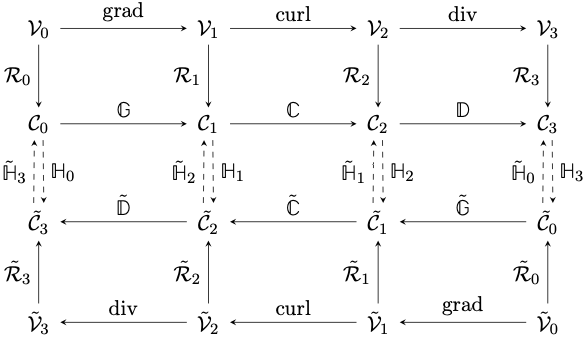
\includegraphics[width=130mm]{deRhamCGL.png}
       \caption{3D de Rham diagram}% Captions are necessary for references to work
       \label{fig:CGL_again}
    \end{figure}

    \item
    table labels should be of the form
    \verb|{tab:*}|
    \begin{table}[htbp]
          \caption{Table example \label{tab:tableEx}}
       \centering\begin{tabular}{c|c|c}
          Bread & Topping 1 & Topping 2 \\ \hline
          Rye & ham & mayonnaise\\
          Corn & ice cream & ketchup\\
       \end{tabular}
    \end{table}

\end{itemize}


\subsection{Using Admonitions in LaTeX Documentation Files}
\label{sec:admonitions_in_latex}

The following admonitions can be used to highlight additional or important information:
\begin{note}
   \verb|\begin{note} \end{note}|
\end{note}
\begin{tip}
   \verb|\begin{tip} \end{tip}|
\end{tip}
\begin{hint}
   \verb|\begin{hint} \end{hint}|
\end{hint}
\begin{attention}
   \verb|\begin{attention} \end{attention}|
\end{attention}
\begin{caution}
   \verb|\begin{caution} \end{caution}|
\end{caution}
\begin{warning}
   \verb|\begin{warning} \end{warning}|
\end{warning}
\begin{danger}
   \verb|\begin{danger} \end{danger}|
\end{danger}
\begin{error}
   \verb|\begin{error} \end{error}|
\end{error}


\subsection{Using Images in LaTeX Documentation Files}
\label{sec:images_in_latex}

Images and other binary files are not supposed to be added to the repository directly. They are instead hosted on the MPCDF Datashare and automatically downloaded to the \textbf{source directory} \verb|doc/sphinx/_static/graphics| when the documentation is built.

From the LaTeX files, images can be included via their relative path, e.g.,
\verb|\includegraphics[width=\linewidth]{../_static/graphics/Examples/ColdPlasma_Dispersion.png}|
results in

\begin{figure}
   \centering
   \includegraphics[width=\linewidth]{../_static/graphics/Examples/ColdPlasma_Dispersion.png}
\end{figure}

\begin{caution}
   The graphics folder is only downloaded if it does not exist locally. If you added new images to the Datashare you have to delete the \textbf{source directory} \verb|doc/sphinx/_static/graphics| or run \verb|make -B| in \verb|$CMAKE_BINARY_DIR/doc| to force the download. Deleting all the build files is not sufficient!
\end{caution}

\end{document}
